\subsubsection{Árboles de decisión} ~\\
\label{subsection:arboles_decision}

%Dado que las características en un clasificador Naive Bayes son independientes entre %sí luego, representar el mismo a través de un árbol de decisión es un buena idea. %Esto se debe a que cada rama es 

Desde el punto de vista de las ciencias de la computación y las matemáticas, un
árbol es un grafo conexo simple y sin ciclos, y sus propiedades son básicas de
la teoría de grafos. Formalmente, un grado es una estructura de la forma $G=(V,E)$, donde $V$ es un conjunto de vértices o nodos y $E=\{ (v_i, v_j), v_j,v_i \in V \}$ es un
conjunto de pares donde cada par representa una arista o rama que conecta a dos nodos.

%	Además, definimos un \textit{camino} o \textit{path} entre los nodos $v_i, v_j \in V, i \neq j$ en $G$ (lo denotamos $P_{v_i, v_j}^G$), como el conjunto $\{ v_i, v_{i+1}, \dots, v_{j-1}, v_j \}$ de nodos talque  $(v_k, v_{k+1}) \in E, k = i, \dots, (j-1)$. Luego, decimos que $G$ es conexo si $\forall v_i, v_j \in V, i \neq j, \exists P_{v_i, v_j}^G$ y no tiene ciclos si $\forall v_i, v_j \in V, i \neq j, \exists ! P_{v_i, v_j}^G $.

	En un árbol existen dos tipos de nodos. La diferencia radica en la cantidad de nodos adyacente al mismo o grado del nodo, que denotamos $d(v_i), v_i \in V$. Los nodos con grado $\leq 1$ se denominan hojas y el resto son nodos internos. Los árboles que consideramos en este trabajo tienen un tercer tipo de nodo que llamamos raíz. Los árboles con raíz son muy comunes en el área de aprendizaje automático y formalmente se pueden definir en términos de \textit{generaciones} o \textit{niveles}. Es decir, consideramos al nodo raíz como el nivel 0, los vecinos del mismo constituyen el primer nivel y los que están a distancia $k$, forman el $k$-esimo nivel.

	Los árboles, en el área de la computación, son estructuras de datos capaces de almacenar y representar información de forma jerárquica (a través de sus nodos). En general y en especial en el área de aprendizaje supervisado son de mucha utilidad ya que computacionalmente son eficientes a la hora de buscar información dentro de ellos (a diferencia de otras estructuras de datos). Además, su representación es fácil de interpretar y su implementación es sencilla.

	Consideremos la Figura \ref{fig: Arbol de decision} que contempla el siguiente problema: ¿Es conveniente ir a jugar al tenis basado en las condiciones climáticas?. La figura es una representación de un árbol de decisión que tiene un estructura similar a un diagrama de flujo. Como se puede observar, en cada nodo del árbol se evalúa un atributo diferente. En este caso, cada atributo hace referencia a una condición climática. En base a la respuesta del nodo raíz se avanza en el árbol hasta llegar a una hoja donde se toma una decisión. En el ejemplo de la figura, si el clima está despejado y la humedad es normal entonces es conveniente ir a jugar al tenis. Los árboles de decisión pueden ser usados para la clasificación (variables discretas) o regresión (variables continuas). Cuando son usados para la clasificación, cada nodo representa una característica, cada rama que sale de un nodo representa un valor posible para la característica que representa al mismo y por último las hojas representan la etiqueta de clase (decisión tomada luego de computar todos los nodos). La clasificación comienza en la raíz, donde se pregunta sobre algún valor de una característica en particular del objeto a analizar. Las diferentes ramas que salen de la  raíz corresponden a las diferentes valores posibles. Basado en la respuesta se continua por la rama hasta el nodo siguiente. La siguiente etapa, es realizar una decisión en el nodo en cuestión que puede ser considerado como la raíz del sub-árbol y se continua de esta manera hasta que se alcanza una hoja, la cual no contiene más preguntas. Cada hoja contiene una etiqueta categórica y al objeto, se le asigna la etiqueta de la hoja que ha alcanzado.
	
		\begin{figure}[htbp]
			\centering
			\fbox{ 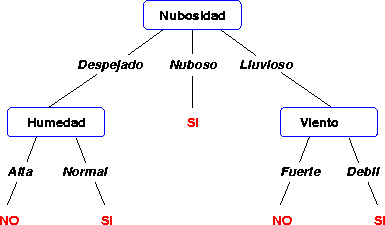
\includegraphics[scale=0.5]{img/tenis_decision_tree.png} }
			\caption{Árbol de decisión.}
			\label{fig: Arbol de decision}
		\end{figure}
		
	Los algoritmos para entrenar un árbol de decisión usualmente trabajan de \textit{arriba hacia abajo}(\textit{top-down}, por su denominación en inglés). Dado un conjunto de características iniciales, en cada nodo del árbol, los algoritmos utilizan una función que evalúa cual es el atributo más apropiado para representar al nodo y en base a eso dividen el conjunto inicial en dos o más partes. La elección de que función utilizar para realizar estas decisiones no es sencilla. En algunos casos, lo que se busca es generar un árbol de decisión óptimo que reduzca el error de generalización, en otros, se busca reducir el número de nodos o la profundida del árbol. Este proceso continúa de manera recursiva hasta que el subconjunto de características en un nodo tiene el mismo valor para la variable objetivo (sea una clase o un valor numérico) o cuando las divisiones no agregan ningún valor a las predicciones. Este proceso es una estrategia muy común al momento de entrenar un árbol de decisión a partir de datos y es un ejemplo de \textit{algoritmo ambicioso}(\textit{greedy algorithm}, por su traducción al inglés). Si se considera nuevamente el ejemplo de la figura \ref{fig: Arbol de decision}, se puede ver que los atributos (si bien son pocos) están bien ubicados en los nodos del árbol. En cambio, si se intercambian los nodos con los atributos \textit{humedad} y \textit{viento}, entonces el preguntar por la humedad sabiendo que el día está lluvioso no aporta información al momento de tomar una decisión.
	
	Lo que se puede destacar, es que cada algoritmo tiene su propio método al momento de dividir el nodo y decidir cual es la mejor división que conlleve a disminuir los errores de clasificación. Por ejemplo, los algoritmos \textit{ID3 y C4.5} \cite{QuinlanID3, QuinlanC45} (el primero es precursor del segundo)  utilizan el concepto de \textit{entropía} o \textit{entropía de información} para elegir al atributo que va a dividir el conjunto de características y que obviamente va a representar al nodo en el árbol. La entropía se la define como la medida de incertidumbre de una variable aleatoria.  Básicamente, dado un conjunto de características $S$, se itera sobre cada atributo no usado del mismo y se calcula la entropía sobre el mismo de la siguiente manera:
	\begin{align}
		\eta(S) = -\sum_i P(s_i)log_{2}P(s_i)
	\end{align}
	donde $S$ es nuestro conjunto conformado con los posibles valores $\{ s_1,\dots, s_n \}$ y $P( \cdot )$ es la función de probabilidad.
	
	Posteriormente, se elige aquel atributo que tenga menor entropía (mayor ganancia de información) y se lo utiliza para partir el conjunto $S$. Construir un árbol de decisión se basa en encontrar atributos que retornen la mayor ganancia de información con lo cual se obtienen ramas más homogéneas.
	
	Los árboles de decisión crecen hasta que se cumplen ciertos criterios algunos de los cuales son: que se haya alcanzado la máxima profundidad del árbol, todas las instancias del conjunto de entrenamiento pertenezcan a un solo valor de salida, entre otros.

	Se puede dar el caso de que el árbol resultante sea excesivamente complejo, por ejemplo, al tener demasiados parámetros relativos al número de observaciones. Esto es lo que se conoce como \textit{sobreajuste} (\textit{overfitting}, de su traducción al inglés). Un modelo que ha sido sobreajustado, tendrá generalmente una baja tasa de predicción. Este tipo de problemas se generan cuando se eligen pobremente los criterios de parada. El caso contrario generaría árboles pequeños o débilmente ajustados.
	
	Una forma de solucionar el sobreajuste es utilizando la técnica de \textit{poda} (\textit{pruning}, de su traducción al inglés). La poda reduce el tamaño de los árboles de decisión eliminando secciones del mismo que provean poca capacidad para clasificar instancias. El objetivo es tanto la reducción de la complejidad del clasificador como así también mejorar la performance a través de la reducción del sobreajuste.
	
	%La entropía, se la define como la medida de incertidumbre en una variable aleatoria y usualmente es medida en \textit{bits, nats o bans}. Para entender el concepto, consideremos el siguiente ejemplo: procedemos a tirar una moneda, si las probabilidades de que salga cara o cruz en la misma son iguales, es decir, la moneda es ``justa'' entonces decimos que la entropía es alta. Dicho de otra manera, no hay forma de predecir con anticipación cual va a ser el resultado. En cambio, si la moneda estuviese alterada y tuviese dos caras entonces la entropía es nula o cero lo cual nos quiere decir que la salida puede ser predecida perfectamente. Formalmente, se define la entropía $\eta$ de una variable aleatoria discreta $X$ con posibles valores $\{ x_1,\dots, x_n \}$ y función de probabilidad $P(X)$ de la siguiente manera:
	%\begin{align}
	%	\eta(X) = E[I(X)] = E[-ln(P(X))]
	%\end{align}
	%donde $E$ es el valor esperado e $I$ es el contenido de información de $X$ ($I(X)$ es en sí misma una variable aleatoria). Cuando se considera una muestra finita, podemos escribir:
	%\begin{align}
	%	\eta(X) = \sum_i P(x_i)I(x_i) = -\sum_i P(x_i)log_{b}P(x_i)
	%\end{align}
	%donde $b$ es la base del logaritmo usado (comúnmente se usa $2$, $10$ o el número de Euler $e$)
